\documentclass{article}
\usepackage[utf8]{inputenc}
\usepackage[spanish,mexico]{babel}
\usepackage{csquotes}
\usepackage{caption}
\usepackage{enumitem}
\usepackage{geometry}
\usepackage{mathtools}
\usepackage{multicol}
\usepackage[backend=bibtex]{biblatex}
\usepackage{graphicx}
\usepackage{fancyvrb}
\usepackage{float}
\usepackage{hyperref}

\addbibresource{references.bib}

 \geometry{
 %total={170mm,257mm},
 top=20mm,
 bottom=20mm,
 left=20mm,
 right=20mm
 }

\title{\textbf{Arquitectura de Computadoras} \\ 
  Diseño de	una computadora simple con lógica de control alambrada}
\author{Mario Becerra \\ Luis Daniel Hernández}
\date{Febrero de 2017}

\setlength\parindent{0pt}
\setlength{\parskip}{0.5em}

\begin{document}

\maketitle


\section{Introducción}

El objetivo de este trabajo es comprender claramente la integración de un computador sencillo.  En particular, entender la forma en que las funciones de control gobiernan los demás componentes del sistema. 

Según \cite{Hennessy_2006}, un diseñador o arquitecto de computadoras debe determinar qué atributos son importantes para una nueva computadora y además diseñar la computadora de tal forma que se maximice el desempeño, y al mismo tiempo mantener dentro de un rango los costos. La arquitectura de computadoras se refiere al diseño del proceso que involucra la construcción de los tres aspectos generales de una computadora: repertorio de instrucciones, organización y hardware.

Las computadoras actuales están basadas en el modelo de Von Neumann, o arquitectura de Von Neumann, desarrollado en Princeton en la década de 1940. Para llegar a este modelo, primero John Mauchly y John Eckert construyeron la ENIAC (\textit{Electronic Numerical Integrator And Computer}) con tubos de vacío. Completada en 1946, la ENIAC fue la primera computadora electrónica digital de propósito general. La principal desventaja de la ENIAC era que tenía que ser programada manualmente con cables y apagadores, lo cual hacía muy difícil y tediosa la tarea de hacer programas. Esta tarea podía facilitarse si el programa pudiera ser representado en una forma tal que el programa pudiera ser almacenado junto con los datos. Esta idea se le atribuye a John Von Neumann, un matemático que era consultor en el proyecto de ENIAC. En 1946, Von Neumann y su equipo empezaron el diseño de una computadora con estas características. El modelo de Von Neumann se refiere a una computadora que es construida con estas características \cite{Stallings:2005:COA:1206425}.

El ciclo esencial de cada instrucción en una computadora que sigue el modelo de Von Neumann es \textit{fetch} y \textit{Execute}. Es decir, se lee una instrucción de memoria, se ejecuta y luego se lee otra instrucción, para así seguir indefinidamente.

\section{Desarrollo}

\subsection{Especificaciones del sistema digital}

La computadora desarrollada en este trabajo tiene las siguientes componentes:

\begin{itemize}
    \item MAR (\textit{Memory Address Register}): Registro que direcciona localidades de memoria
    
    \item MBR (\textit{Memory Buffer Register}): Almacena temporalmente el dato leído o el que se va a escribir en memoria.
    
    \item PC (\textit{Program Counter}): Registro que apunta a la siguiente instrucción a ser ejecutada. Tiene guardada la dirección de memoria donde está guardada la siguiente instrucción a ser ejecutada. Ante cada instrucción ejecutada, actualiza su valor acordemente.
    
    \item IR (\textit{Instruction register}): Contiene el código de operación de la instrucción a ejecutar.
    
    \item Unidad de control: Conjunto de compuertas lógicas cuyo objetivo es orquestar las operaciones de la computadora a través de señales binarias que son enviadas a los demás elementos. Estas señales binarias y sus combinaciones determinan qué microoperación debe ejecutarse en qué tiempo.
    
    \item Contador de tiempo (T): Es un registro contador que aumenta su valor con cada pulso del reloj. Se reinicia (se le asigna el valor de $0$) en ciertas instrucciones, e.g., al cargar un dato a un registro. Va conectado a la unidad de control para que en conjunto con las compuertas lógicas se sepa cuándo ejecutar qué microoperación.
    
\end{itemize}
    
Se tienen además las siguientes especificaciones:

\begin{itemize}
  \item
    La longitud de palabra es de ocho bits.
  
  \item
    Se utilizará como RAM una memoria principal de $64 \times 8$ ($2^6$ palabras de $8$ bits cada una).

  \item  
    La computadora puede ejecutar las diez instrucciones que se especifican en la tabla \ref{tab:microoperaciones_maq}. En donde, \textit{dir} es una dirección de memoria, la cual se especifica en la siguiente palabra del formato de instrucción y $N$ es el bit más significativo del registro $B$.

  \item
    Un programa finaliza con una instrucción \textit{GOTO} en esa misma dirección.  El proceso se podrá detener por medio de una interrupción externa.
  
  \item
    El inicio de un programa se realiza por medio de una interrupción externa.

\end{itemize}

\begin{table}[h]
    \centering
    \caption{Microoperaciones que puede ejecutar la computadora creada}
    \begin{tabular}{|l|l|l|}
    \hline
    Código de operación & Mnemónico & Descripción                                                                                  \\ \hline
    00                  & MOVR      & $B \leftarrow A$                                                                             \\ \hline
    01                  & LD \textit{dir}    & $A \leftarrow M[dir]$                                                                        \\ \hline
    02                  & COMPL     & $B \leftarrow \overline{B}$                                                                  \\ \hline
    03                  & INCB      & $ B \leftarrow B + 1$                                                                        \\ \hline
    04                  & ADDR      & $B \leftarrow A + B$                                                                         \\ \hline
    05                  & CLR A     & $A \leftarrow 0$                                                                             \\ \hline
    06                  & SAVE \textit{dir}  & $M[dir] \leftarrow A$                                                                        \\ \hline
    07                  & INCA      & $A \leftarrow A + 1$                                                                         \\ \hline
    08                  & GOTO \textit{dir}  & $PC \leftarrow dir$                                                                          \\ \hline
    09                  & JPN \textit{dir}   & Si $N = 1$, $PC \leftarrow dir$, si $N = 0$ se ejecuta la siguiente instrucción               \\ \hline
    \end{tabular}    
    \label{tab:microoperaciones_maq}
\end{table}


La computadora fue implementada en \textit{Logisim} \cite{Burch_2002}. El diagrama de la implementación se puede ver en la figura \ref{fig:main_logisim}. En ella, están presentadas las componentes descritas anteriormente, es decir; reloj, MBR, MAR, PC, IR, RAM, unidad de control, y los registros $A$ y $B$, además de dos unidades para calcular la suma y el complemento a unos, y las compuertas lógicas necesarias para la ejecución. Se agregó además un \textit{display} de 7 segmentos para mostrar el contador $T$ del tiempo. Las conexiones entre estas componentes están hechas siguiendo las asignaciones directas en la lógica de control. Por ejemplo, en el ciclo \textit{fetch}, PC manda directamente su contenido a MAR, por lo que hay una conexión directa entre ellos. Los detalles de la implementación de las microoperaciones y la lógica de control están en las siguientes subsecciones.


\begin{figure}[ht]
    \centering
    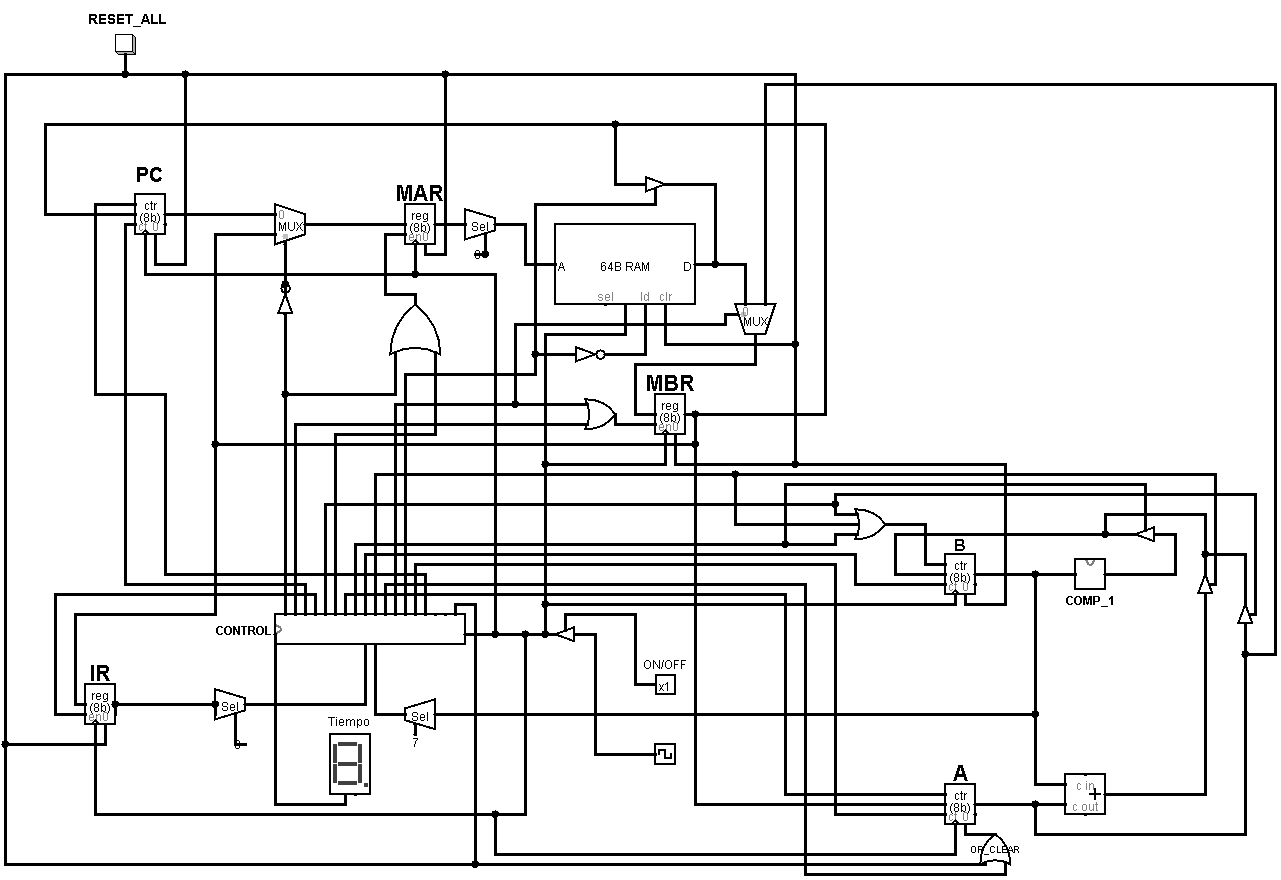
\includegraphics[width=\textwidth]{img/main.png}
    \caption{Computadora implementada en \textit{Logisim}}
    \label{fig:main_logisim}
\end{figure}




\subsection{Microoperaciones}

En la tabla \ref{tab:microoperaciones_tiempos} se presenta el conjunto de microoperaciones de la computadora. Para cada una de las 10 operaciones incluidas en la tabla \ref{tab:microoperaciones_maq}, se muestra la señal necesaria para ejecutar la microoperación. En este caso, $q_i$ se refiere a la $i$-ésima operación de la tabla \ref{tab:microoperaciones_maq} y $t_j$ al $j$-ésimo tiempo guardado en el registro contador $T$. La función \textit{COMPL} se refiere al complemento a unos de la palabra que está guardada en el registro $B$.

\begin{table}[!htbp]
    \fbox{
        \begin{minipage}{\textwidth}
            \begin{multicols}{2}
            
                \begin{itemize}
                    \item \textbf{Fetch}
                        \begin{enumerate}[itemsep=-1ex] 
                            \item[$t_0$:] 
                                MAR $\leftarrow$ PC
                            
                            \item[$t_1$:] 
                                MBR $\leftarrow$ M[MAR], 
                            
                                PC $\leftarrow$ PC + 1
                            
                            \item[$t_2$:] 
                                IR $\leftarrow$ MBR    
                                    
                        \end{enumerate}
                \end{itemize}
                
                
                \begin{itemize}
                    \item \textbf{MOVR}
                        \begin{enumerate}[itemsep=-1ex] 
                            \item[$q_0t_3$:]  
                                B $\leftarrow$ A, 
                                
                                T $\leftarrow$ 0
                        
                        \end{enumerate}
                \end{itemize}
                
                
                \begin{itemize}
                    \item \textbf{LD dir}
                        \begin{enumerate}[itemsep=-1ex] 
                            \item[$q_1t_3$:] 
                            	MAR $\leftarrow$ PC
                            
                            \item[$q_1t_4$:] 
                            	MBR $\leftarrow$ M[MAR],
                            
                            	PC $\leftarrow$ PC + 1
                            
                            \item[$q_1t_5$:] 
                            	MAR $\leftarrow$ MBR
                            
                            \item[$q_1t_6$:] 
                            	MBR $\leftarrow$ M[MAR]
                            
                            \item[$q_1t_7$:] 
                            	A $\leftarrow$ MBR, 
                            
                            	T $\leftarrow$ 0
                        \end{enumerate}
                \end{itemize}
                
                
                
                
                \begin{itemize}
                    \item \textbf{COMPL}
                        \begin{enumerate}[itemsep=-1ex]  
                            \item[$q_2t_3$:] 
                                B $\leftarrow$ COMPL(B),
                                
                                T $\leftarrow$ 0
                    \end{enumerate}
                \end{itemize}
                
                
            
                
                \begin{itemize}
                    \item \textbf{INCB}
                        \begin{enumerate}[itemsep=-1ex] 
                            \item[$q_3 t_3$:]  
                                B $\leftarrow$ B + 1,
                                
                                T $\leftarrow$ 0
                                
                                
                        
                        \end{enumerate}
                \end{itemize}
                
                
                
                
                \begin{itemize}
                    \item \textbf{ADDR}
                        \begin{enumerate}[itemsep=-1ex] 
                            \item[$q_4t_3$: ]  
                                B $\leftarrow$ A + B,
                                
                                T $\leftarrow$ 0
                        
                        \end{enumerate}
                \end{itemize}
                
                
                
                \begin{itemize}
                    \item \textbf{CLR A}
                        \begin{enumerate}[itemsep=-1ex] 
                            \item[$q_5t_3$:]  
                                A $\leftarrow$ 0,
                                
                                T $\leftarrow$ 0
                        
                        \end{enumerate}
                \end{itemize}
            
                
                
                \begin{itemize}
                    \item \textbf{SAVE dir}
                        \begin{enumerate}[itemsep=-1ex] 
                            \item[$q_6t_3$:]  
                                MAR $\leftarrow$ PC
                            
                            \item[$q_6t_4$:]
                                MBR $\leftarrow$ M[MAR],
                                
                                PC $\leftarrow$ PC + 1
                            
                            \item[$q_6t_5$:]
                                MAR $\leftarrow$ MBR
                   
                            \item[$q_6t_6$:] 
                                MBR $\leftarrow$ A
                            
                            \item[$q_6t_7$:] 
                                M[MAR] $\leftarrow$ MBR,
                                
                                T $\leftarrow$ 0
                        
                        \end{enumerate}
                \end{itemize}
                
            
            
                \begin{itemize}
                    \item \textbf{INCA}
                        \begin{enumerate}[itemsep=-1ex] 
                            \item[$q_7 t_3$:]  
                                A $\leftarrow$ A + 1,
                                
                                T $\leftarrow$ 0
                                
                        
                        \end{enumerate}
                \end{itemize}
                
                
                
                \begin{itemize}
                    \item \textbf{GOTO dir}
                        \begin{enumerate}[itemsep=-1ex] 
                            \item[$q_8t_3$:] 
                                MAR $\leftarrow$ PC
                            
                            \item[$q_8t_4$:]
                                MBR $\leftarrow$ M[MAR]
                                
                            \item[$q_8t_5$:]
                                PC $\leftarrow$ MBR,
                    
                                T $\leftarrow$ 0
                        \end{enumerate}
                \end{itemize}
                
                
                
                
                \begin{itemize}
                    \item \textbf{JPN dir}
                        \begin{enumerate}[itemsep=-1ex] 
                            \item[$q_9t_3$:]
                                MAR $\leftarrow$ PC
                            
                        \item[$q_9t_4$:] 
                            MBR $\leftarrow$ M[MAR],
                            
                            PC $\leftarrow$ PC + 1
                   
                        \item[$q_9t_5\overline{N}$:]
                            T $\leftarrow$ 0
                        
                        \item[$q_9t_5N$:]
                            PC $\leftarrow$ MBR,
                            
                            T $\leftarrow$ 0
                        
                        \end{enumerate}
                \end{itemize}
            
            \end{multicols}
        
        \end{minipage}
    
    }

    \caption{Microoperaciones de la computadora}
    \label{tab:microoperaciones_tiempos}
\end{table}

\newpage

\subsection{Unidad de control}

A partir de las operaciones y tiempos anteriores, se crean las siguientes señales para que la unidad de control funcione.

\begin{itemize}

  \item MAR $\leftarrow$ PC: $X_1 = t_0 + q_1 t_3 + q_6 t_3 + q_8 t_3 + q_9 t_3$

  \item MBR $\leftarrow$ M[MAR]: $X_2 = t_1 + q_1 t_4 + q_1 t_6 + q_6 t_4 + q_8 t_4 + q_9 t_4$

  \item PC $\leftarrow$ PC + 1: $X_3 = t_1 + q_1 t_4 + q_6 t_4 + q_9 t_4$

  \item IR $\leftarrow$ MBR: $X_4 = t_2 $

  \item B $\leftarrow$ A: $X_5 = q_0 t_3$

  \item MAR $\leftarrow$ MBR: $X_6 = q_1 t_5 + q_6 t_5$

  \item A $\leftarrow$ MBR: $X_7 = q_1 t_7$

  \item B $\leftarrow$ COMP(B): $X_8 = q_2 t_3$

  \item B $\leftarrow$ B + 1: $X_9 = q_3 t_3$

  \item B $\leftarrow$ A + B: $X_{10} = q_4 t_3$

  \item A $\leftarrow$ 0: $X_{11} = q_5 t_3$

  \item MBR $\leftarrow$ A: $X_{12} = q_6 t_6$

  \item M[MAR] $\leftarrow$ MBR: $X_{13} = q_6 t_7$

  \item A $\leftarrow$ A + 1: $X_{14} = q_7 t_3$

  \item PC $\leftarrow$ MBR: $X_{15} = q_8 t_5 + q_9 t_5 N$

  \item $X_{16} = q_9 t_5 \overline{N}$

  \item T $\leftarrow$ 0: $X_{17} = X_5 + X_7 + X_8 + X_9 + X_{10} + X_{11} + X_{13} + X_{14} + X_{15} + X_{16}$

\end{itemize}

La unidad de control se puede ver implementada en la figura \ref{fig:control_logisim}. Donde se tienen dos decodificadores, uno de ellos conectado al IR y otro al reloj; se tiene $N$, que es el bit más significativo del registro $B$, un contador $T$ que aumenta con los pulsos del reloj; y compuertas lógicas que dan como salida 17 señales que son utilizadas en el resto de la computadora para ejecutar las microoperaciones. Estas 17 señales corresponden a las $X_1, \hdots, X_{17}$ que se acaban de definir.

\begin{figure}[h]
    \centering
    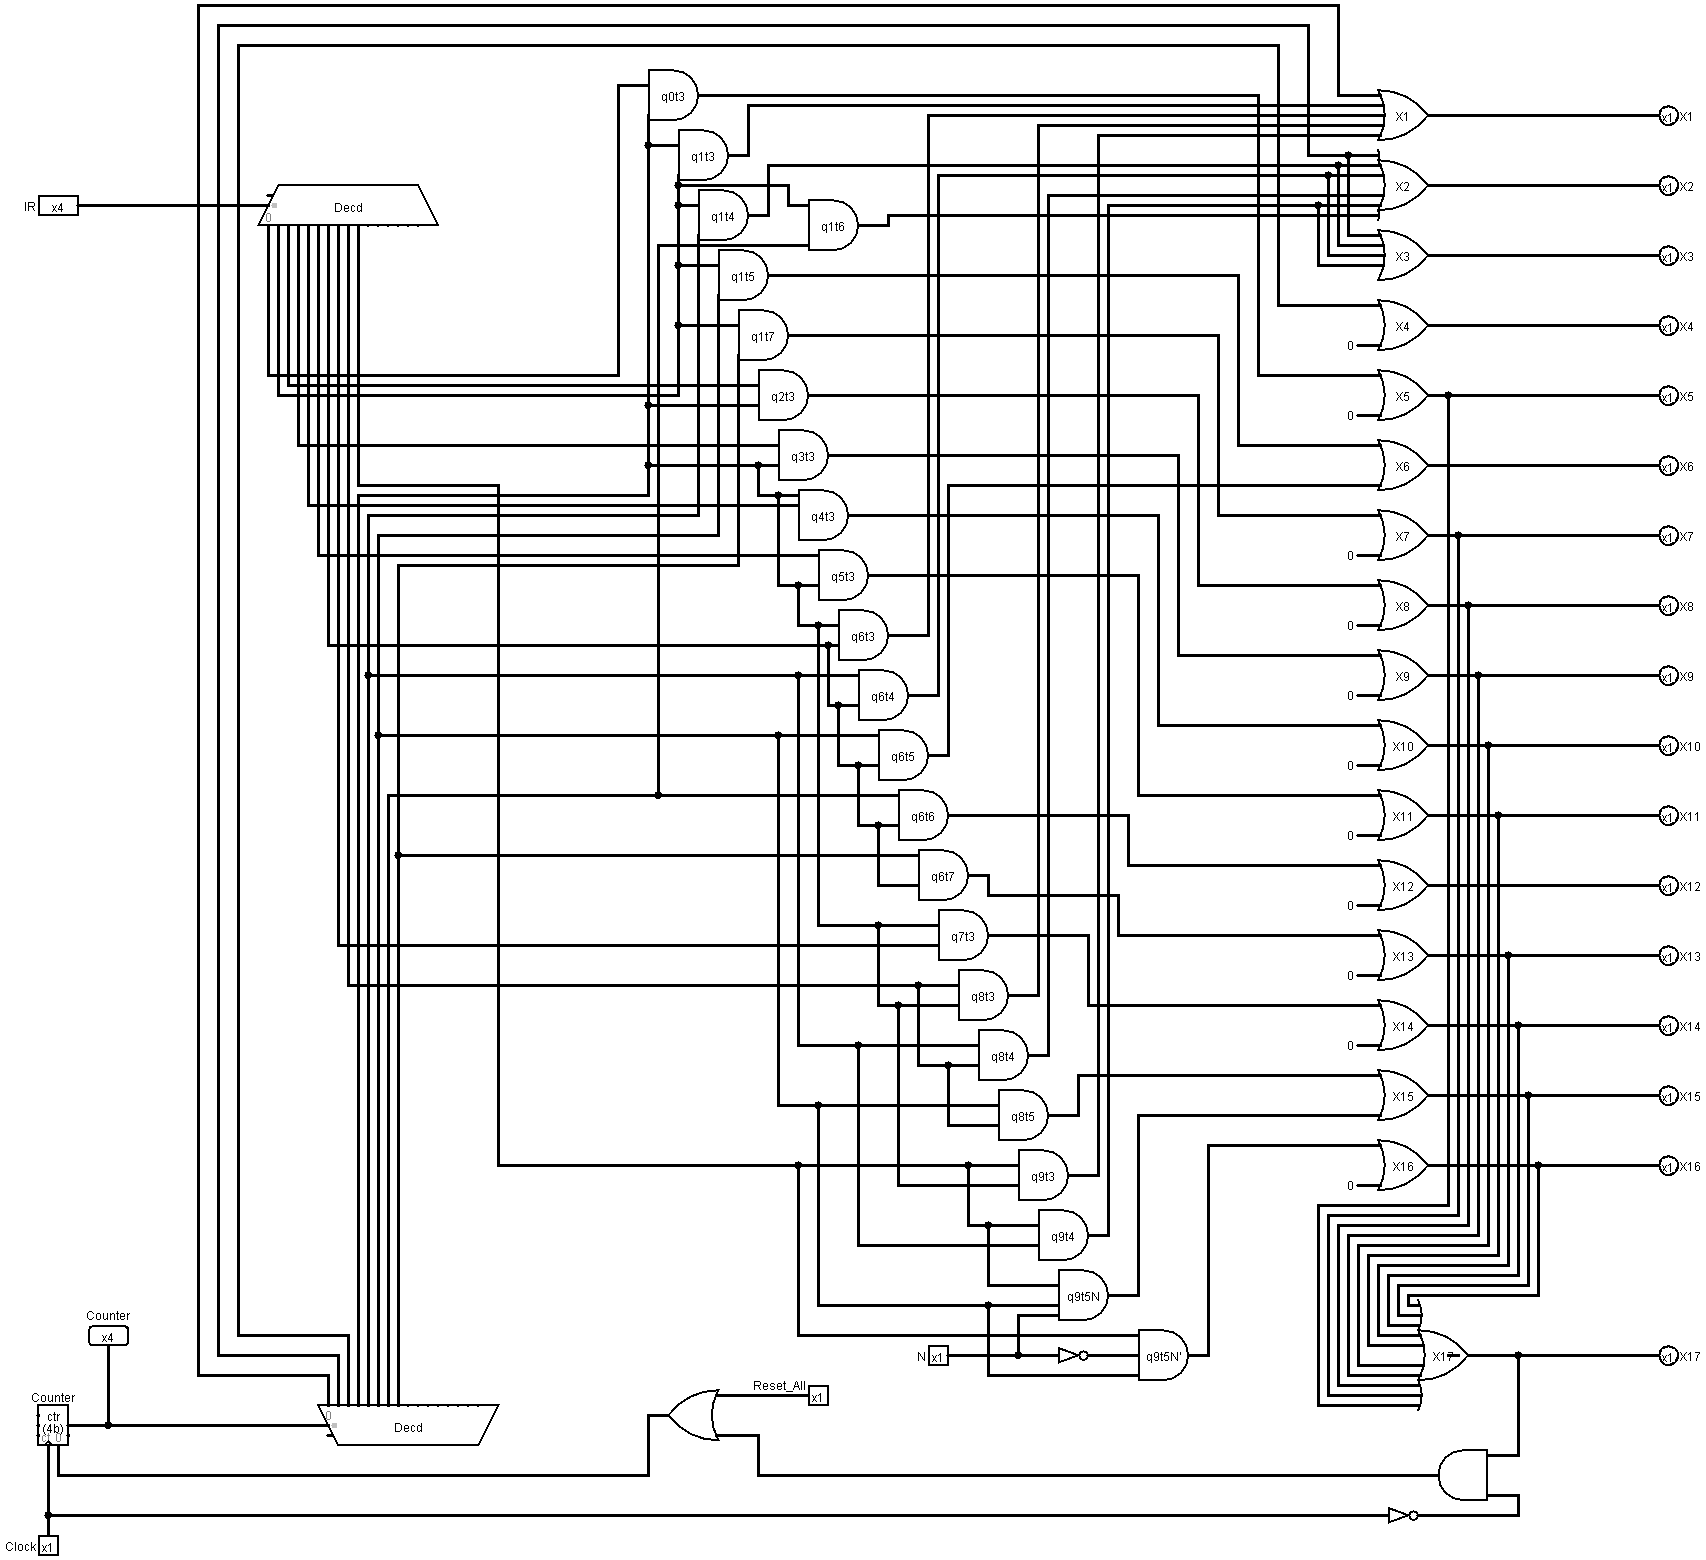
\includegraphics[width=\textwidth]{img/control.png}
    \caption{Unidad de control alambrada implementada en \textit{Logisim}}
    \label{fig:control_logisim}
\end{figure}

\section{Simulación de código de alto nivel}

Con las instrucciones de la computadora anterior, se diseñó un programa en un pseudo lenguaje ensamblador para ejecutar el siguiente operador ternario de C.

\begin{verbatim}
    x = (x < y) ? 0 : x + 1    
\end{verbatim}

Se asume que \texttt{x} se encuentra en la localidad de memoria $20$, \texttt{y} en la $21$ y que el programa se carga a partir de la localidad $0$.

El código en el pseudo lenguaje ensamblador que ejecuta el operador ternario es el siguiente:

\begin{Verbatim}[numbers=left,xleftmargin=5mm]
    LD 20;
    MOVR;
    LD 21;
    COMPL;
    INCB;
    ADDR:
    JPN L1; 
    CLRA;
    SAVE 20;
    GOTO L2;
    
    L1:
    LD 20;
    INCA;
    SAVE 20;
    GOTO L2;
    
    L2:
    GOTO L3;
    
    L3:
    GOTO L2;
\end{Verbatim}

La primera instrucción carga en el registro $A$ el valor que está en la dirección de memoria $20$, es decir, el valor de \texttt{x}. Posteriormente, se mueve el valor del registro $A$ al registro $B$, para a continuación cargar en el registro $A$ el valor de la dirección de memoria $21$, es decir, \texttt{y}. La cuarta instrucción calcula el complemento a uno del registro $B$, para que en la quinta incremente su valor en $1$; esto es equivalente a calcular el complemento a dos del registro $B$, lo cual a su vez es lo mismo que multiplicar \texttt{y} por $-1$. La instrucción 6 suma los valores del registro $A$ y del registro $B$ para guardarlos en el registro $B$ (es decir, calcula \texttt{x - y}).

La instrucción $7$ es la esencia del \texttt{if}, pues si el bit más significativo de $B$ es igual a $0$, significa que \texttt{x > y}. En ese caso sigue ejecutando las instrucciones que siguen, es decir, \texttt{CLRA} y \texttt{SAVE 20}, las cuales \emph{resetean} el registro $A$ y guardan ese valor en la localidad de memoria $20$, i.e., hacen \texttt{x = 0}.

Por el otro lado, si el bit más significativo de $B$ es igual a $1$, significa que \texttt{x < y}. En la sintaxis de este pseudo lenguaje ensamblador, se le indica que brinque a la sección \texttt{L1} para ejecutar las instrucciones que están en las líneas 13 a 16. Lo que se está haciendo en la computadora, es brincar a la dirección $50$ (elegido arbitrariamente), para cargar en el registro $A$ el valor de la localidad de memoria $20$ (\texttt{LD 20}), incrementar el valor del registro $A$ (\texttt{INCA}) y guardar el resultado en la localidad $20$, es decir, se hace \texttt{x = x + 1}.

Finalmente, en ambos casos, en las líneas 10 y 16, se manda a la sección \texttt{L2}, la cual manda a la sección \texttt{L3}, quien manda a la sección \texttt{L3}, etc.; es decir, se cicla. 

A continuación, se presentan los registros de la memoria RAM en la computadora una vez que se guarda el programa para ejecutar la condición ternaria. Cada número de dos dígitos es un número hexadecimal que representa una instrucción, una dirección o un valor. La localidad 0 es la que está hasta la izquierda en la línea 1, la localidad 2 es la que le sigue a la derecha, y así sucesivamente hasta llegar a la localidad 63 que es la que está hasta la derecha en la línea 8.

\begin{Verbatim}[numbers=left,xleftmargin=5mm]
    01 14 00 01 15 02 03 04
    09 32 05 06 14 08 0c 00
    00 00 00 00 f8 f4 00 00
    00 00 00 00 00 00 00 00
    00 00 00 00 00 00 00 00
    00 00 00 00 00 00 00 00
    00 00 01 14 07 06 14 08
    37 00 00 00 00 00 00 00
\end{Verbatim}

Para ejecutar el programa, el PC debe contener el número 0 pues se asume que el programa empieza en la localidad 0. Lo primero que se hace es ejecutar el ciclo \textit{fetch} y mandar al IR la instrucción \texttt{01} (\texttt{LD}), la cual carga el valor de la dirección de memoria \texttt{0x14} (20 en notación decimal) en el registro $A$. La localidad 2 tiene la instrucción \texttt{00}, esto significa que debe ejecutar el \texttt{MOVR}. Las localidades 3 y 4 indican que se haga un \texttt{LD} de la dirección \texttt{0x15} (21 en decimal) en el registro $A$. La localidad 5 manda ejecutar el complemento a uno del registro $B$ (\textit{opcode} \texttt{02}) para luego en la 6 incrementar el valor de $B$ (\textit{opcode} \texttt{03}). Posteriormente, en la 7 se ejecuta la suma de los registros $A$ y $B$ (\textit{opcode} \texttt{04}). 

En la localidad 8 se ejecuta el \texttt{JPN} (\textit{opcode} \texttt{09}). En caso de que \texttt{N} sea 0, se ejecuta la siguiente instrucción de memoria que está en la localidad 10, en otro caso, brinca a la localidad \texttt{0x32} (50 en decimal).

La localidad 10 tiene el valor de \texttt{05}, por lo que si \texttt{N} es 0, se ejecutará el comando \texttt{CLRA} y posteriormente \texttt{SAVE} en la localidad \texttt{0x14} (20 en decimal). Después, en la localidad 13, se manda a llamar un \texttt{GOTO} a la misma localidad 13 (\texttt{0x0c} en decimal) para ciclar el programa y darlo por terminado.

En el caso que \texttt{N} sea 1, el PC se actualiza con el valor \texttt{0x32} (50 en decimal) y ejecuta un \texttt{LD} (\textit{opcode} \texttt{01}) de la localidad 20 (\texttt{0x14} en hexadecimal). En la localidad 52 hace un incremento (\texttt{INCA}, \textit{opcode} \texttt{07}) y después \texttt{SAVE} en la localidad \texttt{0x14} (20 en decimal). Finalmente, en la localidad 55, se manda a llamar un \texttt{GOTO} a la misma localidad 55 (\texttt{0x37} en decimal) para ciclar el programa y darlo por terminado.

\section{Conclusiones}

El diseño de una computadora, incluso una sencilla como la mostrada aquí, es una tarea complicada y laboriosa que no debe ser tomada a la ligera. Hay muchos detalles que se tienen que tomar en cuenta que si no se toman con el debido cuidado pueden hacer que la funcionalidad se venga abajo. Este trabajo ayudó a que tomáramos en cuenta esos detalles y pudiéramos abstraer mucho mejor las tareas que hacen las computadoras.

Si se desea probar la computadora creada, se puede acceder a ella en \\ \url{https://github.com/mariobecerra/ComputerArchitecturePP1}.

\printbibliography
\nocite{*}


\end{document}
